%% -*- coding: utf-8 -*-
\documentclass[pdftex,aspectratio=169]{beamer}

%% -*- coding: utf-8 -*-
\usetheme{Boadilla} % default
\useoutertheme{infolines}
\setbeamertemplate{navigation symbols}{} 

\usepackage{etex}
\usepackage{alltt}
\usepackage{pifont}
\usepackage{color}
\usepackage[utf8]{inputenc}
%\usepackage{german}
\usepackage{listings}
\lstset{language=Haskell}
\lstset{sensitive=true}
\usepackage{hyperref}
\hypersetup{colorlinks=true}
\usepackage[final]{pdfpages}
\usepackage{url}
\usepackage{arydshln} % dashed lines
\usepackage{tikz}
\usepackage{mathpartir}

\DeclareUnicodeCharacter{3BB}{\ensuremath{\lambda}}


\newcommand\cmark{\ding{51}}
\newcommand\xmark{\ding{55}}

\newcommand{\nat}{\mathbf{N}}

\usepackage[all]{xy}

%% new arrow tip for xy
\newdir{|>}{!/4.5pt/@{|}*:(1,-.2)@^{>}*:(1,+.2)@_{>}}

\newcommand\cid[1]{\textup{\textbf{#1}}} % class names
\newcommand\kw[1]{\textup{\textbf{#1}}}  % key words
\newcommand\tid[1]{\textup{\textsf{#1}}} % type names
\newcommand\vid[1]{\textup{\texttt{#1}}} % value names
\newcommand\Mid[1]{\textup{\texttt{#1}}} % method names

\newcommand\TODO[1][]{{\color{red}{\textbf{TODO: #1}}}}

\newcommand\String[1]{\texttt{\dq{}#1\dq{}}}

\newcommand\ClassHead[1]{%
  \ensuremath{\begin{array}{|l|}
      \hline
      \cid{#1}
      \\\hline
    \end{array}}}
\newcommand\AbstractClass[2]{%
  \ensuremath{\begin{array}{|l|}
      \hline
      \cid{\textit{#1}}
      \\\hline
      #2
      \hline
    \end{array}}}
\newcommand\Class[2]{%
  \ensuremath{\begin{array}{|l|}
      \hline
      \cid{#1}
      \\\hline
      #2
      \hline
    \end{array}}}
\newcommand\Attribute[3][black]{\textcolor{#1}{\Param{#2}{#3}}\\}
\newcommand\Methods{\hline}
\newcommand\MethodSig[3]{\Mid{#2} (#3): \,\tid{#1}\\}
\newcommand\CtorSig[2]{\Mid{#1} (#2)\\}
\newcommand\AbstractMethodSig[3]{\Mid{\textit{#2}} (#3): \,\tid{#1}\\}
\newcommand\Param[2]{\vid{#2}:~\tid{#1}}

\lstset{%
  frame=single,
  xleftmargin=2pt,
  stepnumber=1,
  numbers=left,
  numbersep=5pt,
  numberstyle=\ttfamily\tiny\color[gray]{0.3},
  belowcaptionskip=\bigskipamount,
  captionpos=b,
  escapeinside={*'}{'*},
  language=java,
  tabsize=2,
  emphstyle={\bf},
  commentstyle=\mdseries\it,
  stringstyle=\mdseries\rmfamily,
  showspaces=false,
  showtabs=false,
  keywordstyle=\bfseries,
  columns=fullflexible,
  basicstyle=\footnotesize\CodeFont,
  showstringspaces=false,
  morecomment=[l]\%,
  rangeprefix=////,
  includerangemarker=false,
}

\newcommand\CodeFont{\sffamily}

\definecolor{lightred}{rgb}{0.8,0,0}
\definecolor{darkgreen}{rgb}{0,0.5,0}
\definecolor{darkblue}{rgb}{0,0,0.5}

\newcommand\highlight[1]{\textcolor{blue}{\emph{#1}}}
\newcommand\GenClass[2]{\cid{#1}\texttt{<}\cid{#2}\texttt{>}}

\newcommand\Colored[3]{\alt<#1>{\textcolor{#2}{#3}}{#3}}

\newcommand\nt[1]{\ensuremath{\langle#1\rangle}}

\newcommand{\free}{\operatorname{free}}
\newcommand{\bound}{\operatorname{bound}}
\newcommand{\var}{\operatorname{var}}
\newcommand\VSPBLS{\vspace{-\baselineskip}}

\newcommand\IF{\textit{IF}}
\newcommand\TRUE{\textit{TRUE}}
\newcommand\FALSE{\textit{FALSE}}

\newcommand\IFZ{\textit{IF0}}
\newcommand\ZERO{\textit{ZERO}}
\newcommand\SUCC{\textit{SUCC}}
\newcommand\ADD{\textit{ADD}}
\newcommand\SUB{\textit{SUB}}
\newcommand\MULT{\textit{MULT}}
\newcommand\DIV{\textit{DIV}}

\newcommand\PAIR{\textit{PAIR}}
\newcommand\FST{\textit{FST}}
\newcommand\SND{\textit{SND}}

\newcommand\CASE{\textit{CASE}}
\newcommand\LEFT{\textit{LEFT}}
\newcommand\RIGHT{\textit{RIGHT}}

\newcommand\Encode[1]{\lceil#1\rceil}
\newcommand\Reduce{\stackrel\ast\rightarrow_\beta}

\newcommand\Nat{\textit{Nat}}
\newcommand\Bool{\textit{Bool}}
\newcommand\Pair{\textit{Pair}}
\newcommand\Tfun[1]{#1\to}

\newcommand\Tenv{A}
\newcommand\Lam[1]{\lambda#1.}
\newcommand\App[1]{#1\,}
\newcommand\Succ{\textit{SUCC}\,}
\newcommand\Let[2]{\textit{let}\,#1=#2\,\textit{in}\,}

\newcommand\calE{\mathcal{E}}
\newcommand\calU{\mathcal{U}}
\newcommand\calP{\mathcal{P}}
\newcommand\calW{\mathcal{W}}

\newcommand\GEN{\textit{gen}}
\newcommand\EFV[1]{\textit{fv} (#1)}
\newcommand\Dom[1]{\textit{dom} (#1)}

%%% Local Variables: 
%%% mode: latex
%%% TeX-master: nil
%%% End: 

%%% frontmatter
%% -*- coding: utf-8 -*-

\title{Functional Programming}
\subtitle{Introduction}

\author[Peter Thiemann]{Prof. Dr. Peter Thiemann}
\institute[Univ. Freiburg]{Albert-Ludwigs-Universität Freiburg, Germany}
\date{SS 2019}


\subtitle
{Lambda Calculus}

\begin{document}

\begin{frame}
  \titlepage
\end{frame}

%\begin{frame}
%  \frametitle{Outline}
%  \tableofcontents
  % You might wish to add the option [pausesections]
%\end{frame}


\begin{frame}[fragile]
  \frametitle{The Lambda Calculus}
\begin{block}<+->{What Wikipedia says}
  \href{https://en.wikipedia.org/wiki/Lambda_calculus}{Lambda
    calculus} (also written as λ-calculus) is a formal system in
  mathematical logic for expressing computation based on function
  abstraction and application [\dots]. It is a universal model of
  computation that can be used to simulate any Turing machine and was
  first introduced by mathematician Alonzo Church in the 1930s as part
  of his research [on] the foundations of mathematics.  
\end{block}
\begin{block}<+->{Further down it says}
  \begin{itemize}
  \item[\textcolor{green}\cmark] Lambda calculus has applications in many different areas in mathematics, philosophy, linguistics, and computer science.
  \item[\textcolor{green}\cmark] Lambda calculus has played an important role in the development of the theory of programming languages.
  \item[\textcolor{red}\xmark] Functional programming languages implement the lambda calculus.
  % \item Lambda calculus also is a current research topic in Category theory.
  \end{itemize}
\end{block}
\end{frame}             

\begin{frame}[fragile]
  \frametitle{Syntax of the λ-calculus}
  \begin{block}<+->{λ terms}
    \begin{align*}
      M,N & ::= x & \text{variable} \\
          & \mid (\lambda x. M) & \text{(lambda) abstraction} \\
          & \mid (M\, N) & \text{application}
    \end{align*}
    \begin{itemize}
    \item Variables are drawn from infinite denumerable set
    \item $(\lambda x. M)$ \textbf{binds} $x$ in $M$
    \end{itemize}
  \end{block}
  \begin{block}<+->{Conventions for omitting parentheses}
    \begin{itemize}
    \item abstractions extend as far to the right as possible
    \item application is left associative
    \end{itemize}
  \end{block}
\end{frame}             

\begin{frame}[fragile]
  \frametitle{Working with lambda terms}
  \begin{block}{Free and bound variables}
    \begin{align*}
    \free(x) & = \{ x \} \\
    \free(M\,N) & = \free(M) \cup \free(N) \\
    \free(\lambda x.M) & = \free(M) \setminus \{x\}\\[1ex]
    \bound(x) & = \varnothing\\
    \bound(M\,N) & = \bound(M) \cup \bound(N) \\
      \bound(\lambda x.M) & = \bound(M) \cup \{x\} \\[1ex]
      \var (M) & = \free (M) \cup \bound (M)
    \end{align*}
    A  lambda term $M$ is \textbf{closed} ($M$ is a
    \textbf{combinator}) iff $\free(M)=\varnothing$. \\
    Otherwise the term is
  \textbf{open}. 
  \end{block}
\end{frame}

\begin{frame}[fragile]
  \frametitle{Working with lambda terms}
  \begin{block}{Substitution $M[x\mapsto N]$}
    \vspace{-\baselineskip}
    \begin{alignat*}{2}
    x[x\mapsto N] & = N\\
    y[x\mapsto N] & = y \quad & x\neq y\\
    (\lambda x.M)[x\mapsto N] & := \lambda x.M\\
    (\lambda y.M)[x\mapsto N] & := \lambda y.(M[x\mapsto N])
    \quad & x\neq y, y\not\in\free(N)\\
    (\lambda y.M)[x\mapsto N] & := \lambda y'.(M[y\mapsto y'][x\rightarrow N])
    \quad & x\neq y, y\in\free(N), y'\not\in\free(M)\cup\free(N)\\
    (M\,M')[x\mapsto N] & := (M[x\mapsto N])(M'[x\mapsto N])
  \end{alignat*}
\end{block}
\begin{alertblock}{Guiding principle: \textbf{capture freedom}}
  In every $(\lambda x.M)$ the bound variable $x$ is ``connected'' to each
  free occurrence of $x$ in $M$. These connections must not be broken by
  substitution. 
\end{alertblock}
\end{frame}             


\begin{frame}[fragile]
  \frametitle{Computing with lambda terms}
  \begin{block}<+->{Reduction rules}\VSPBLS
    \begin{alignat*}{2}
      (\lambda x.M) & \rightarrow_{\alpha} (\lambda y.M[x\mapsto y]) \quad 
      & y\not\in\free(M) & \quad\text{Alpha reduction}
      \\
      ((\lambda x.M)\,N) & \rightarrow_{\beta} M[x\mapsto N]
      && \quad\text{Beta reduction (\textcolor{red}{function application})}
      \\
      (\lambda x.(M\,N)) & \rightarrow_{\eta} M \quad
      & x\not\in\free(M) & \quad \text{Eta reduction}
    \end{alignat*}
  \end{block}
  \begin{block}<+->{Reductions may be applied everywhere in a term}
    \begin{displaymath}
    \begin{array}{c}
      M \rightarrow_x M'
      \\\hline
      (\lambda y.M) \rightarrow_x (\lambda y.M')
    \end{array}
    \qquad
    \begin{array}{c}
      M \rightarrow_x M'
      \\\hline
      (M~N) \rightarrow_x (M'~N)
    \end{array}
    \qquad
    \begin{array}{c}
      N \rightarrow_x N'
      \\\hline
      (M~N) \rightarrow_x (M~N')
    \end{array}
  \end{displaymath}
  \end{block}
\end{frame}

\begin{frame}[fragile]
  \frametitle{The theory of the lambda calculus}
  \begin{alertblock}<+->{Computation and equivalence}
    For $x\subseteq\{\alpha,\beta,\gamma\}$ and reduction relation $\rightarrow_x$,
    \begin{itemize}
    \item $\stackrel{\ast}{\rightarrow}_x$ is the reflexive-transitive
      closure,
    \item $\leftrightarrow_x$ is its symmetric closure,
    \item $\overset{\ast}{\leftrightarrow}_x$ is its
      reflexive-transitive-symmetric closure.
    \end{itemize}
  \end{alertblock}
  \begin{alertblock}<+->{Equality in lambda calculus}
    \begin{itemize}
    \item Alpha equivalence: $M =_\alpha N$ iff $M
      \overset{\ast}{\leftrightarrow}_{\alpha} N$.
    \item Standard: $M =_\beta N$ iff $M
      \overset{\ast}{\leftrightarrow}_{\alpha,\beta} N$.
    \item Extensional: $M =_{\beta\eta} N$ iff $M
      \overset{\ast}{\leftrightarrow}_{\alpha,\beta,\eta} N$.
    \end{itemize}
  \end{alertblock}
\end{frame}             


\begin{frame}[fragile]
  \frametitle{Computing with lambda terms}
  \begin{alertblock}<+->{Definition: Normal form}
    Let $M$ be a lambda term. \\
    A lambda term $N$ is a \textbf{normal
      form} of $M$ iff $M\overset{\ast}{\rightarrow}_\beta N$ and there
    is no $N'$ with $N\rightarrow_\beta N'$.
  \end{alertblock}
  \begin{block}<+->{}
    Lambda terms with equivalent (equal modulo $\alpha$ reduction) normal
    forms exhibit the same behavior.
    The reverse is not always true.
  \end{block}
  \begin{alertblock}<+->{A lambda term without normal form}
    \begin{displaymath}
  (\lambda x.x~x)(\lambda x.x~x) \rightarrow_\beta (\lambda
  x.x~x)(\lambda x.x~x) 
\end{displaymath}
  \end{alertblock}
\end{frame}             

\begin{frame}[fragile]
  \frametitle{Computing with lambda terms makes sense}
  \begin{alertblock}<+->{The Church-Rosser theorem}
    Beta reduction has the \textbf{Church-Rosser property}:
    \begin{center}
      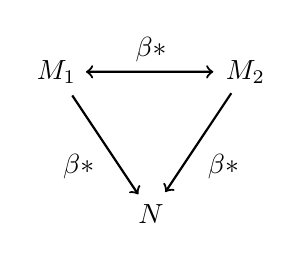
\begin{tikzpicture}[scale=0.6,shorten >=1pt, auto]
        \node (M1) at (2,5) {$M_1$} ;
        \node (M2) at (6,5) {$M_2$} ;
        \node (N) at (4,2) {$N$} ;
        \draw
        (M1) edge[<->,thick] node {$\beta\ast$} (M2)
        (N) edge[<-, thick] node {$\beta\ast$} (M1)
        (M2) edge[->, thick] node {$\beta\ast$} (N)
        ;
      \end{tikzpicture}
    \end{center}
    That is: For
    all $M_1, M_2$ with
  $M_1 \overset{\ast}{\leftrightarrow}_\beta M_2$,
  there is some $N$ with
  $M_1\overset{\ast}{\rightarrow}_\beta N$ and
  $M_2\overset{\ast}{\rightarrow}_\beta N$.
\end{alertblock}
\begin{block}<+->{Corollary}
  A lambda term $M$ has at most one normal form modulo $\alpha$
  reduction.
\end{block}
\end{frame}


\begin{frame}[fragile]
  \Huge
  \begin{center}
    {Programming in the pure lambda calculus}
  \end{center}
\end{frame}



\begin{frame}[fragile]
  \frametitle{From functions to arbitrary datatypes}
  \begin{block}{Any computation may be encoded in the lambda calculus}
    \begin{itemize}
    \item Booleans and conditionals
    \item Numbers
    \item Recursion
    \item Products (pairs)
    \item Variants
    \end{itemize}
  \end{block}
\end{frame}             

\begin{frame}[fragile]
  \frametitle{Booleans and conditional}
  \begin{exampleblock}<+->{Requirements / Specification}
    Wanted: Lambda terms $\IF$, $\TRUE$, $\FALSE$ such that
    \begin{itemize}
    \item $\IF~\TRUE~M\,N \stackrel\ast\rightarrow_\beta M$
    \item $\IF~\FALSE~M\,N \stackrel\ast\rightarrow_\beta N$
    \end{itemize}
  \end{exampleblock}
  \begin{exampleblock}<+->{Idea}
    $\TRUE$ and $\FALSE$ are functions that select the first or second
    argument, respectively
  \end{exampleblock}
  \end{frame}

\begin{frame}
  \frametitle{Booleans and conditional}
  \begin{block}<+->{Booleans}\VSPBLS
    \begin{align*}
      \TRUE &= \lambda x.\lambda y.x &
      \FALSE &= \lambda x.\lambda y.y
    \end{align*}
  \end{block}
  \begin{block}<+->{Conditional}\VSPBLS
    \begin{align*}
      \IF &= \lambda b.\lambda t.\lambda f. b\,t\,f
    \end{align*}
  \end{block}
  \begin{alertblock}<+->{Check the spec!}
    \dots
  \end{alertblock}
\end{frame}


\begin{frame}[fragile]
  \frametitle{Natural numbers}
  \begin{exampleblock}{Requirements / Specification}
    Wanted: A family of lambda terms $\lceil n\rceil$, for each
    $n\in\nat$, such that the arithmetic operations are \emph{lambda
      definable}.

    That is, there are lambda terms $\ADD$, $\SUB$, $\MULT$, $\DIV$ such that
    \begin{itemize}
    \item $\ADD~\Encode m~\Encode n \Reduce \Encode{m+n}$
    \item $\SUB~\Encode m~\Encode n \Reduce \Encode{m-n}$
    \item $\MULT~\Encode m~\Encode n \Reduce \Encode{mn}$
    \item $\DIV~\Encode m~\Encode n \Reduce \Encode{m/n}$
    \end{itemize}
  \end{exampleblock}
\end{frame}

\begin{frame}[fragile]
  \frametitle{Church numerals}
\begin{exampleblock}<+->{One approach}
  % Numbers can be represented in several different ways by lambda
  % terms.  One is to use \textbf{Church numerals}.
  The \textbf{Church numeral}
  $\Encode{ n}$ of some natural number $n$ is a function that takes
  two parameters, a function $f$ and some $x$, and applies $f$ $n$-times to $x$.
\end{exampleblock}
\begin{alertblock}<+->{Zero}\VSPBLS
  \begin{align*}
    \Encode{0} & = \lambda f. \lambda x. x
  \end{align*}
\end{alertblock}
\begin{alertblock}<+->{Successor}\VSPBLS
  \begin{align*}
    \SUCC & = \lambda n. \lambda f. \lambda x. f (n\, f\,x)
  \end{align*}
\end{alertblock}
\end{frame}

\begin{frame}[fragile]
  \frametitle{Church numerals --- addition and multiplication}
\begin{alertblock}<+->{Addition}\VSPBLS
  \begin{align*}
    \ADD & = \lambda m. \lambda n. \lambda f. \lambda x. m\, f (n\, f\, x)
  \end{align*}
\end{alertblock}
\begin{alertblock}<+->{Multiplication}\VSPBLS
  \begin{align*}
    \MULT & = \lambda . \lambda n. \lambda f. \lambda x. m\, (n\, f)\, x
  \end{align*}
\end{alertblock}
\end{frame}

\begin{frame}[fragile]
  \frametitle{Church numerals --- conditional}
  \begin{exampleblock}<+->{Wanted}
    $\IFZ$ such that
    \begin{itemize}
    \item $\IFZ~\Encode 0~M~N \Reduce M$
    \item $\IFZ~\Encode n~M~N \Reduce M$ if $n\ne 0$
    \end{itemize}
  \end{exampleblock}
  \begin{alertblock}<+->{Testing for zero}\VSPBLS
    \begin{align*}
      \IFZ &= \lambda n. \lambda z. \lambda s. n\,(\lambda x. s)\,z
    \end{align*}
  \end{alertblock}
  \begin{alertblock}<+->{Check the spec!}
    \dots
  \end{alertblock}
\end{frame}




\begin{frame}
  \frametitle{Pairs}
  \begin{exampleblock}<+->{Specification}
    Wanted: lambda terms $\PAIR$, $\FST$, $\SND$ such that
    \begin{itemize}
    \item $\FST (\PAIR~M~N) \Reduce M$
    \item $\SND (\PAIR~M~N) \Reduce N$
    \end{itemize}
  \end{exampleblock}
  \begin{alertblock}<+->{Implementation}\VSPBLS
    \begin{align*}
      \PAIR &= \lambda x.\lambda y. \lambda v. v\,x\,y \\
      \FST  &= \lambda p. p (\lambda x.\lambda y. x) \\
      \SND  &= \lambda p. p (\lambda x.\lambda y. y)
    \end{align*}
  \end{alertblock}
\end{frame}

\begin{frame}
  \frametitle{Variants (Either)}
  \begin{exampleblock}<+->{Specification}
    Wanted: lambda terms $\LEFT$, $\RIGHT$, $\CASE$ such that
    \begin{itemize}
    \item $\CASE (\LEFT~M) N_l\,N_r \Reduce N_l\,M$
    \item $\CASE (\RIGHT~M) N_l\,N_r \Reduce N_r\,M$
    \end{itemize}
  \end{exampleblock}
  \begin{alertblock}<+->{Implementation}\VSPBLS
    \begin{align*}
      \CASE &= \\
      \LEFT &= \\
      \RIGHT&=
    \end{align*}
  \end{alertblock}
\end{frame}
\begin{frame}
  \frametitle{Recursion}
  \begin{alertblock}<+->{Fixpoint theorem}
    Every lambda term has a fixpoint:

    For every $M$ there is some $N$ such that
    $
    M\, N \overset{\ast}{\leftrightarrow}_\beta N
    $.
  \end{alertblock}
  \begin{exampleblock}<+->{Proof}
    Let $N = Y~M$ where
    \begin{displaymath}
      Y := \lambda f.(\lambda x.f~(x~x))~(\lambda x.f~(x~x)).
    \end{displaymath}
  \end{exampleblock}
  \begin{block}{Remark}
    $Y$ is Curry's \textbf{fixpoint combinator}. There are infinitely
    many more fixpoint combinators with various properties.
  \end{block}
\end{frame}
\begin{frame}
  \frametitle{Wrapup}
  \begin{itemize}
  \item Lambda calculus contains the primitives of the theory of
    recursive functions
  \item The theory of recursive functions is Turing complete
  \item Hence is the (untyped) lambda calculus
  \end{itemize}
\end{frame}
\end{document}


